% !TEX root =  ../supplementary.tex
\section{Personalized Biopsies Based on Risk of Reclassification}
Consider some real patients from the PRIAS database shown in Figure~\ref{fig:demo_pat1_supp} to Figure~\ref{fig:demo_pat4_supp}. We intend to develop personalized schedule of biopsies for these patients. Using the joint model fitted to the PRIAS dataset, we first obtain their cumulative risk of reclassification over the entire follow-up period (see Equation~\ref{eq:dynamic_risk_prob}). This cumulative risk accounts for their entire history of PSA as well as the time of their latest negative biopsy. Assume a new patient $j$ whose latest biopsy was conducted at time $t$ and who has visited the clinic at the current time $s$. We suggest a biopsy at his current visit time $s$ if his cumulative risk of reclassification at $s$ given by $R_j(s \mid t)$ (see Section~\ref{sec:param_estimates_jm_fit_prias}) is above a certain threshold (e.g., 10\% risk). Suppose that in this way a decision of biopsy is taken at time $s$. Since patients may be removed from AS upon detection of reclassification, the schedule of remaining future biopsies can only be made under the assumption that reclassification did not happen before time $s$. Under this assumption we update the patient's cumulative risk of reclassification at next visit time $s+1$ to be $R_j(s + 1 \mid s)$. Now, if $R_j(s + 1 \mid s) < 10\%$, then we will not schedule a biopsy at $s+1$. Instead, we will decide for a biopsy at a subsequent time $s + 2$ using the cumulative risk $R_j(s + 2 \mid s)$ at $s+2$. If however, at time $s+1$ the cumulative risk of reclassification $R_j(s + 1 \mid s) \geq 10\%$ then we would have decided for a biopsy at $s+1$. Consequently, the biopsy decision at time $s + 2$ would have been made using the updated cumulative risk $R_j(s + 2 \mid s + 1)$ and not $R_j(s + 2 \mid s)$. We repeat this process for a horizon in each cohort (PRIAS and five external GAP3 cohorts). This horizon is the maximum time point $t_h$, such that there are at least 10 patients who experience reclassification after $t_h$. This horizon is six years in PRIAS. While scheduling these biopsies we always maintain a minimum gap of one year, as recommended in PRIAS. Personalized schedules can also be made with any other risk threshold such as 5\% or 15\%.

To assist patients in making an informed choice for a schedule, be it personalized or fixed, we provide them patient-specific consequences of following each schedule. To this end, we first calculate the probability of occurrence of reclassification between successive biopsies of each schedule. Using these probabilities we then obtain the expected delay in detection of reclassification for following that schedule. Thus, patients have a method to compare across various schedules in terms of the personalized burden (time and total biopsies), and personalized benefit (less delay in detection of reclassification is beneficial). Suppose once again that for patient $j$, the time of latest negative biopsy is $t_0$, and current visit time is $s > t_0$. Then equation for the expected delay $D_j(\mathcal{S} \mid t,s)$ in detection of reclassification using schedule of biopsies $\mathcal{S} = \{t_1, \ldots, t_h\}$, where $t_1 \geq s$, and $t_h$ is the horizon time up to which we want to schedule biopsies, is given by:
\begin{equation}
\label{eq:expected_delay}
\begin{split}
D_j(\mathcal{S} \mid t,s) &= \sum_{v=1}^{h} R_j(t_v\mid t_{v-1},s) \times  \Big\{t_{v} - t_{v-1} - \int_{t_{v-1}}^{t_v} S_j(u \mid t_v, t_{v-1}, s) \mathrm{d}u \Big\},\\
S_j(u \mid t_v, t_{v-1}, s) &= \mbox{Pr}\big\{T^*_j > u \mid t_{v} \geq T^*_j > t_{v-1}, \mathcal{Y}_{j}(s), \mathcal{D}_n\big\}, \quad t_{v} \geq u > t_{v-1},
\end{split}
\end{equation}
and $R_j(t_v\mid t_{v-1},s)$ is as defined in Equation~(\ref{eq:dynamic_risk_prob}). The personalized and fixed schedules, and their consequences for a few real patients from the PRIAS dataset are shown in Figure~\ref{fig:demo_pat1_supp} to Figure~\ref{fig:demo_pat4_supp}. A compulsory biopsy was done at horizon $t_h$ of follow-up in all schedules for meaningful comparison of their expected delays in detection of reclassification.

\begin{figure}
\centerline{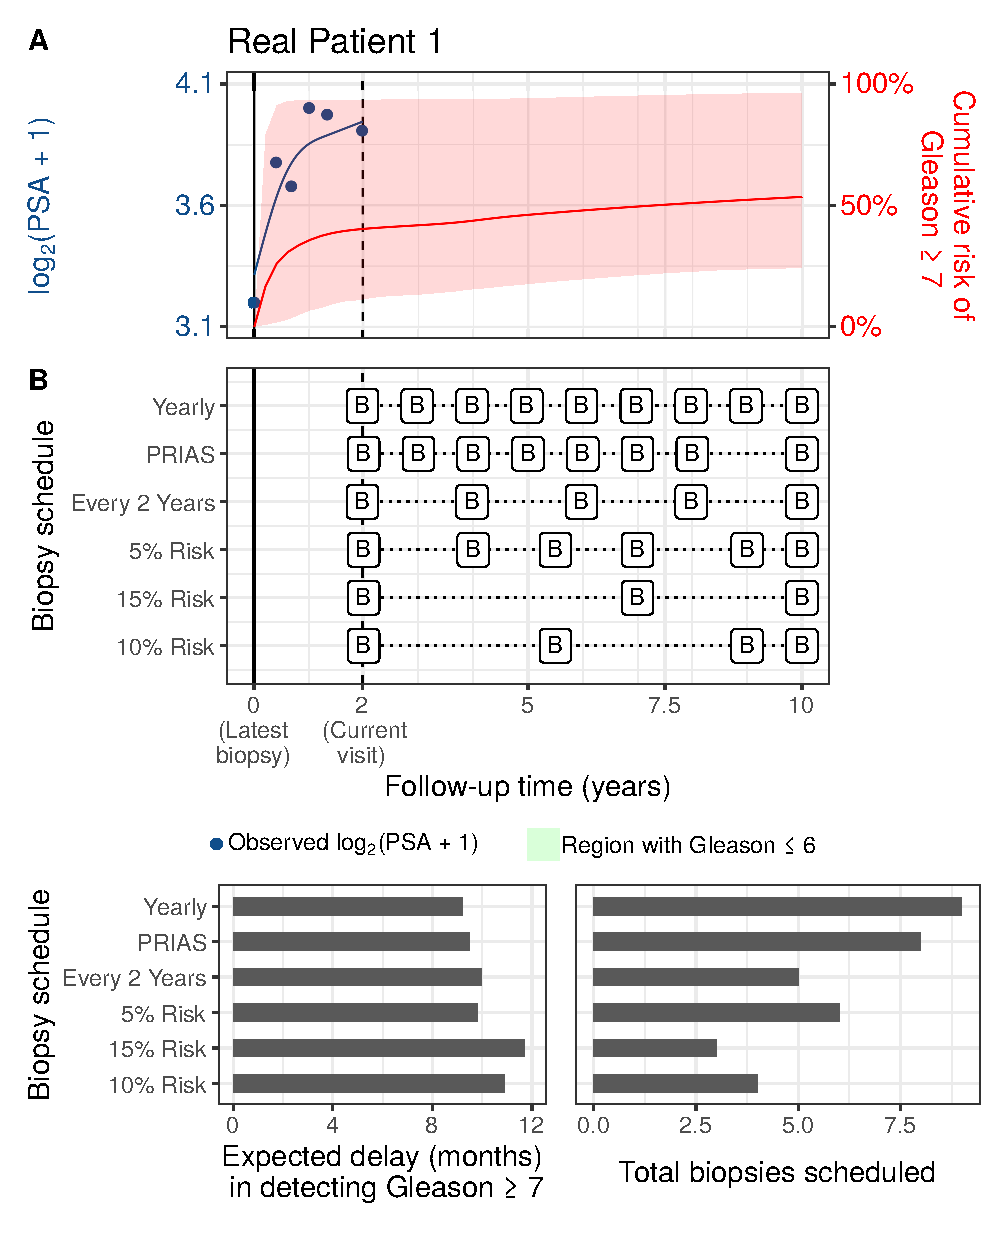
\includegraphics[width=\columnwidth]{images/demo_pat1_supp.eps}}
\caption{\textbf{Personalized and fixed schedules of biopsies for patient 1}. \textbf{Panel~A:} shows the observed and fitted $\log_2(\mbox{PSA} + 1)$ measurements (Equation~\ref{eq:long_model_psa}), and the dynamic cumulative risk of Gleason $\geq$ 7 (see \ref{sec:param_estimates_jm_fit_prias}) over follow-up period. \textbf{Panel~B} shows the personalized and fixed schedules of biopsies with a `B' indicating times of biopsies. In the bottom two panels, the various schedules are compared in terms of the number of biopsies they schedule, and the expected delay in detection of Gleason $\geq$ 7 if they are followed.}
\label{fig:demo_pat1_supp}
\end{figure}

\begin{figure}
\centerline{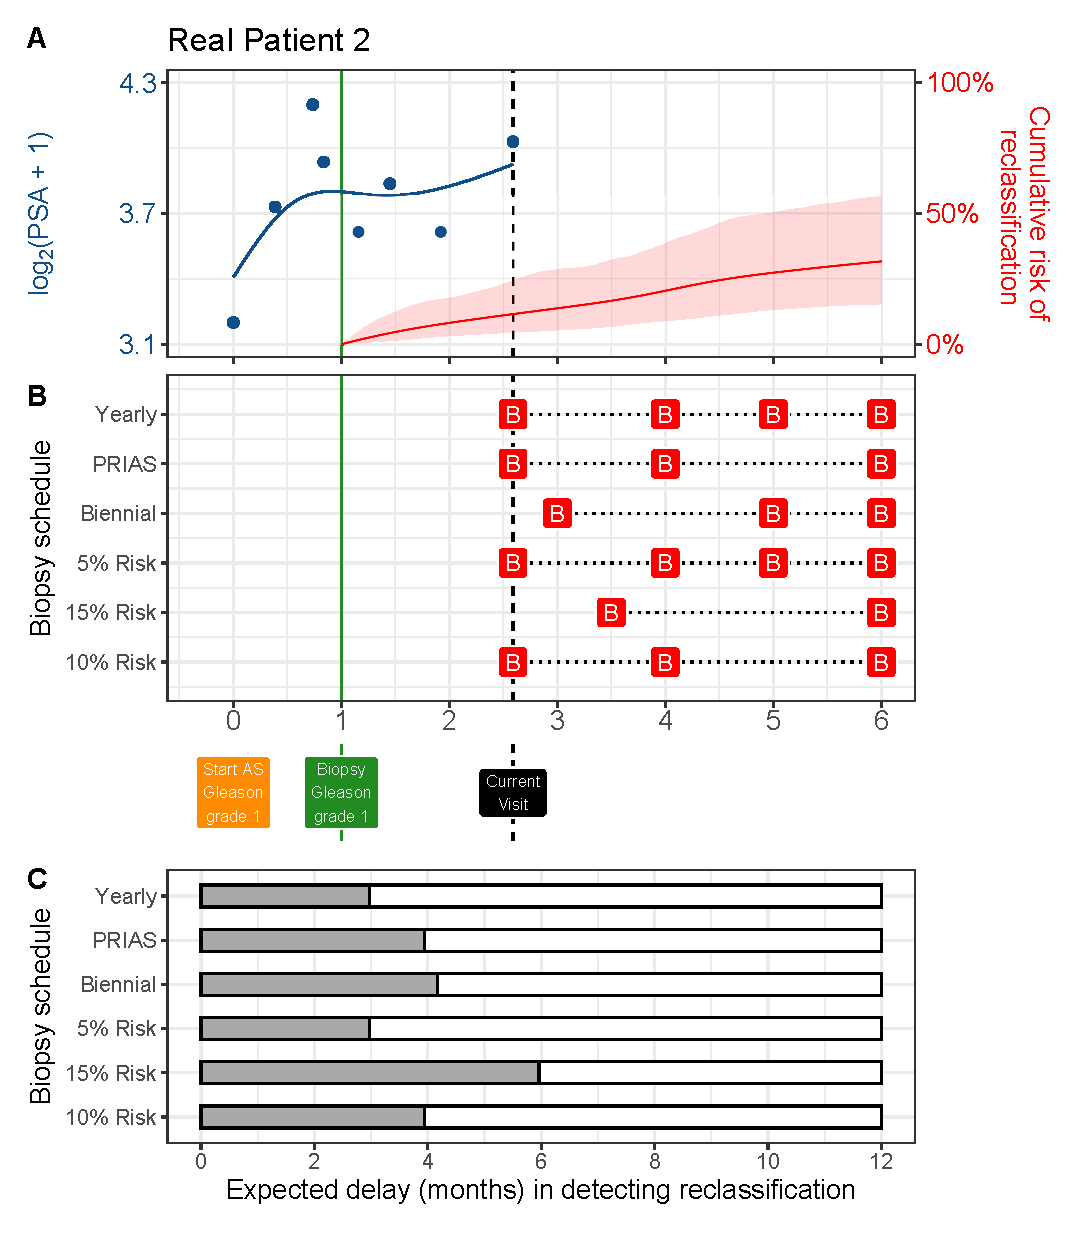
\includegraphics[width=\columnwidth]{images/demo_pat2_supp.eps}}
\caption{\textbf{Personalized and fixed schedules of biopsies for patient 2}. \textbf{Panel~A:} shows the observed and fitted $\log_2(\mbox{PSA} + 1)$ measurements (Equation~\ref{eq:long_model_psa}), and the dynamic cumulative risk of Gleason $\geq$ 7 (see \ref{sec:param_estimates_jm_fit_prias}) over follow-up period. \textbf{Panel~B} shows the personalized and fixed schedules of biopsies with a `B' indicating times of biopsies. In the bottom two panels, the various schedules are compared in terms of the number of biopsies they schedule, and the expected delay in detection of Gleason $\geq$ 7 if they are followed.}
\label{fig:demo_pat2_supp}
\end{figure}

\begin{figure}
\centerline{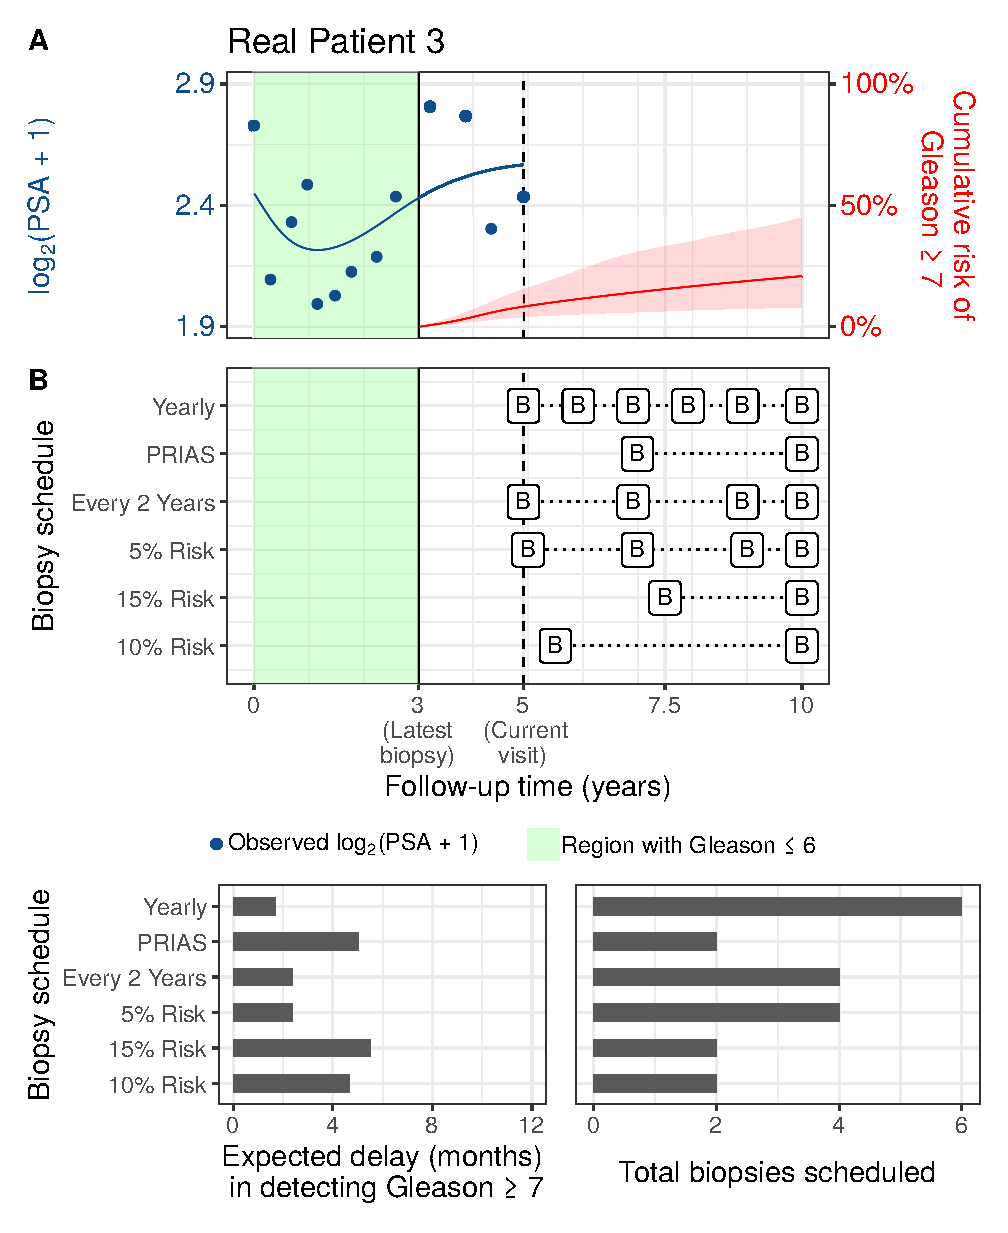
\includegraphics[width=\columnwidth]{images/demo_pat3_supp.eps}}
\caption{\textbf{Personalized and fixed schedules of biopsies for patient 3}. \textbf{Panel~A:} shows the observed and fitted $\log_2(\mbox{PSA} + 1)$ measurements (Equation~\ref{eq:long_model_psa}), and the dynamic cumulative risk of Gleason $\geq$ 7 (see \ref{sec:param_estimates_jm_fit_prias}) over follow-up period. \textbf{Panel~B} shows the personalized and fixed schedules of biopsies with a `B' indicating times of biopsies. In the bottom two panels, the various schedules are compared in terms of the number of biopsies they schedule, and the expected delay in detection of Gleason $\geq$ 7 if they are followed.}
\label{fig:demo_pat3_supp}
\end{figure}

\begin{figure}
\centerline{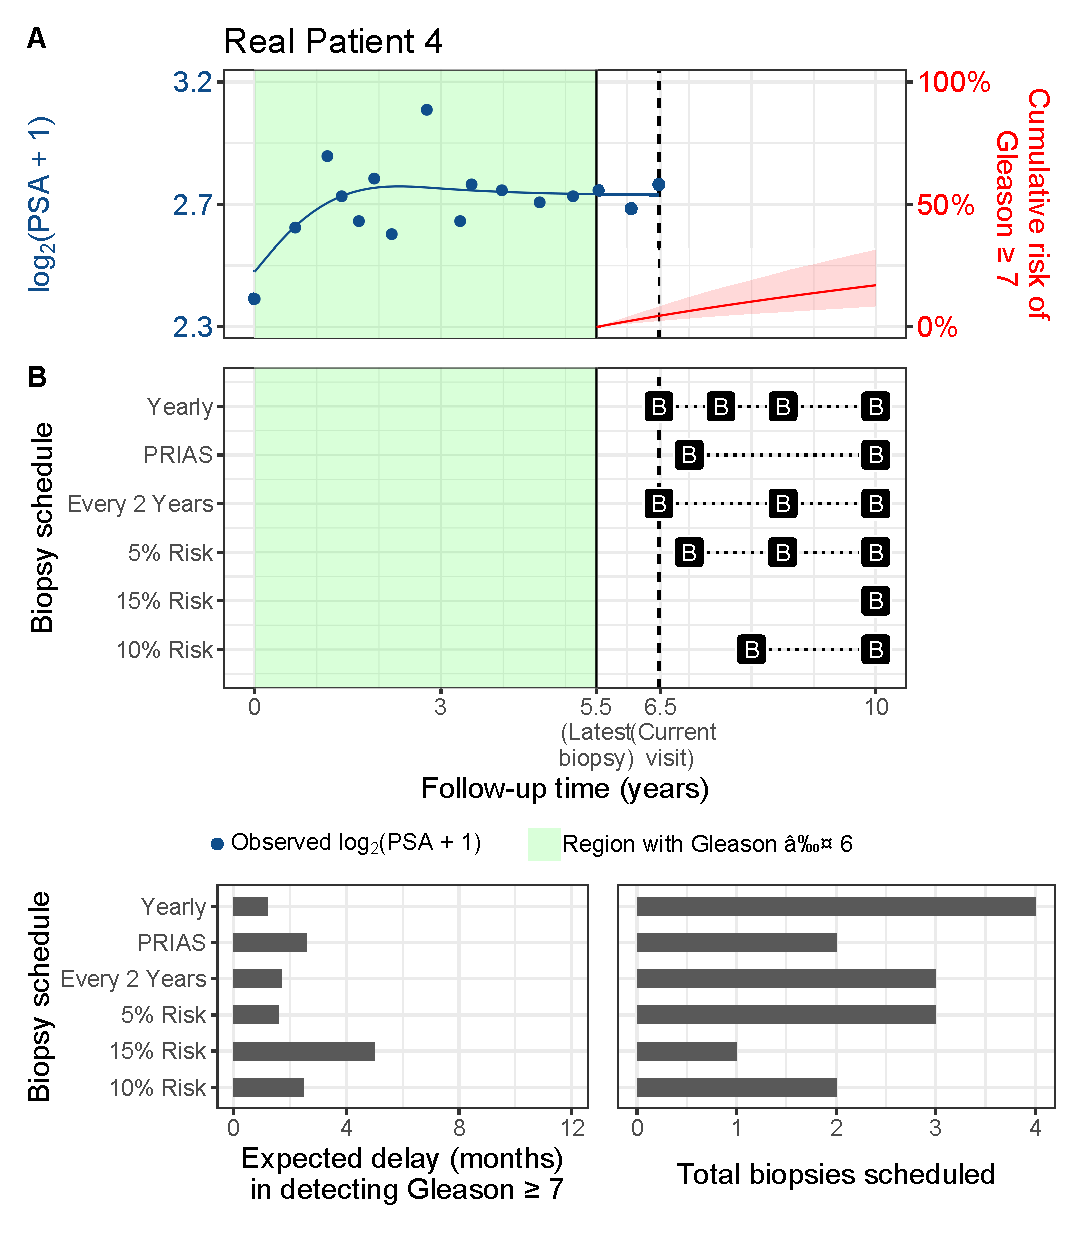
\includegraphics[width=\columnwidth]{images/demo_pat4_supp.eps}}
\caption{\textbf{Personalized and fixed schedules of biopsies for patient 4}. \textbf{Panel~A:} shows the observed and fitted $\log_2(\mbox{PSA} + 1)$ measurements (Equation~\ref{eq:long_model_psa}), and the dynamic cumulative risk of Gleason $\geq$ 7 (see \ref{sec:param_estimates_jm_fit_prias}) over follow-up period. \textbf{Panel~B} shows the personalized and fixed schedules of biopsies with a `B' indicating times of biopsies. In the bottom two panels, the various schedules are compared in terms of the number of biopsies they schedule, and the expected delay in detection of Gleason $\geq$ 7 if they are followed.}
\label{fig:demo_pat4_supp}
\end{figure}